\section{Results}
\subsection{S1: preserved failure and prospective confirmation}
The original S1 development result is unchanged: all 64 IID and 64 coefficient-OOD cases require 63 PCG iterations under both learned and zero starts. The diagnostic tolerance sweep finds an IID benefit of 12.86\% at $10^{-2}$, but an OOD change of $-4.26$\%; the advantage disappears or reverses at more stringent settings. This diagnostic is not substituted for the frozen endpoint.

The original frozen S1 confirmation yields 0.00\% IID and 0.00\% coefficient-OOD mean iteration reduction. Its recorded disposition is \texttt{NEGATIVE}. The source-linear successor is therefore not presented as a successful rerun of S1: it changes the predictor, preconditioning controls and evaluation protocol and uses disjoint data.

\subsection{S2: primary outcome and cost}
Table~\ref{tab:primary} reports the primary cell, with 160 paired cases across five independent training blocks. Table~\ref{tab:comparisons} gives paired effect estimates; a mean of paired ratios differs from a ratio of mean times. The predeclared joint iteration rule is satisfied, producing \texttt{SUPPORTED} for this narrow primary hypothesis. All 17280 successor condition-level rows are retained; 0 fail true-residual acceptance.
\begin{table}[ht]
\centering\small\begin{tabular}{lrrr}
\toprule
Method & Mean iterations & Mean time (ms) & Mean rel. error \\
\midrule
Direct Thomas & 0.000 & 0.448 & 0.00e+00 \\
Zero + Jacobi & 126.069 & 3.246 & 2.20e-10 \\
Quadratic + Jacobi & 126.963 & 3.360 & 6.05e-11 \\
Zero + Laplacian & 12.556 & 3.212 & 2.33e-09 \\
Physics + Laplacian & 11.556 & 3.393 & 3.94e-09 \\
Quadratic + Laplacian & 10.544 & 2.853 & 4.87e-09 \\
Degree 1 + Laplacian & 10.425 & 2.789 & 4.94e-09 \\
Structured + Laplacian & 9.131 & 2.518 & 6.75e-09 \\
Shuffled + Laplacian & 12.619 & 3.326 & 2.58e-09 \\
\bottomrule
\end{tabular}

\caption{Frozen S2 primary cell: IID, 129 grid points, relative tolerance $10^{-6}$. Online time includes assembly, inference, setup, correction and residual certification. Training and loading are excluded.}\label{tab:primary}
\end{table}
\begin{table}[ht]
\centering\small\begin{tabular}{lrrr}
\toprule
Baseline & Iteration reduction & 95\% block interval & Online saving \\
\midrule
Zero + Laplacian & 27.73\% & [27.28, 28.22]\% & 21.72\% \\
Physics + Laplacian & 21.17\% & [20.94, 21.50]\% & 26.07\% \\
Quadratic + Laplacian & 13.58\% & [13.17, 14.00]\% & 11.69\% \\
Shuffled + Laplacian & 28.07\% & [27.33, 28.99]\% & 24.47\% \\
Direct Thomas & -- & -- & -463.63\% \\
\bottomrule
\end{tabular}

\caption{Structured predictor plus Laplacian PCG versus each listed baseline. Negative online saving means slower. Direct solving has no meaningful relative-iteration metric. Five-block bootstrap intervals have limited resolution.}\label{tab:comparisons}
\end{table}
\begin{figure}[ht]
\centering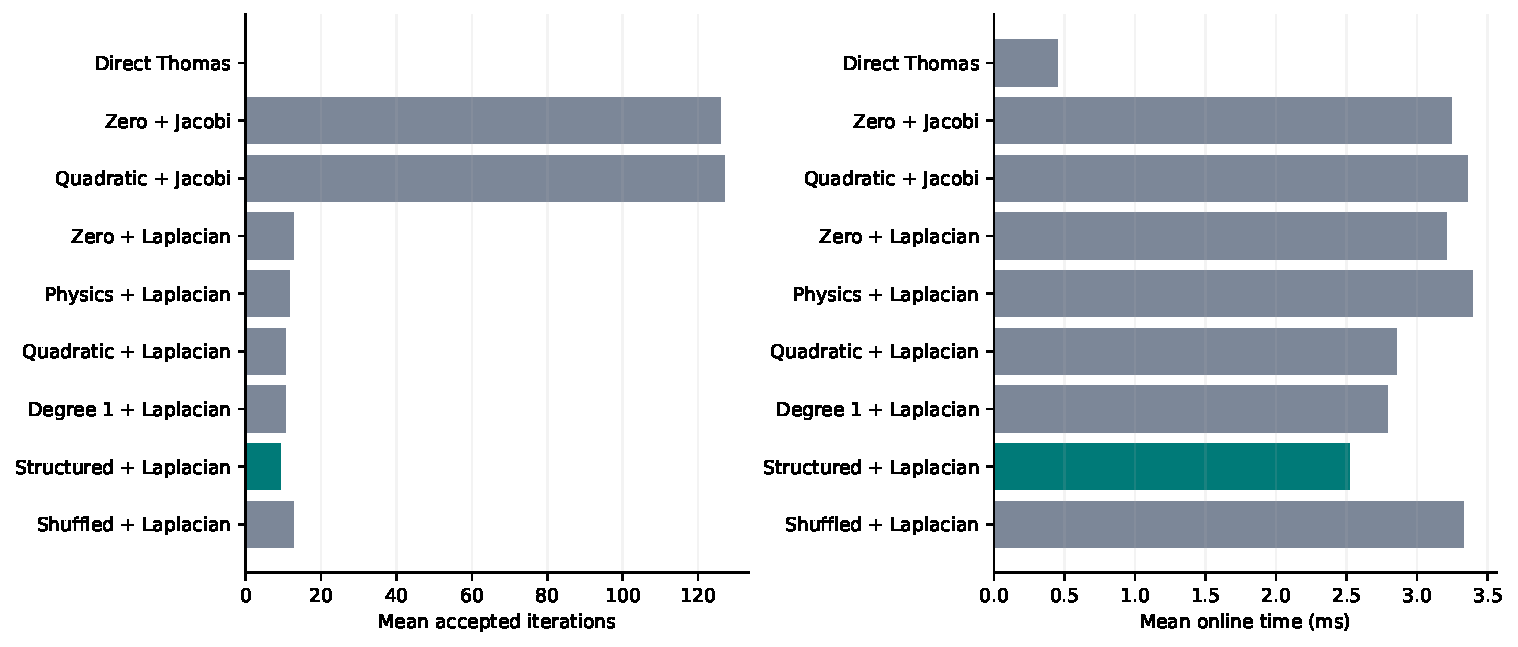
\includegraphics[width=\linewidth]{figures/primary.pdf}
\caption{Accepted correction work and complete online time. The classical preconditioner changes the scale of correction work; direct tridiagonal solving remains the fastest measured path.}\label{fig:primary}
\end{figure}

The direct method is 5.61 times faster than the proposed method by the ratio of mean online times. Therefore the evidence does not support replacing direct 1D solving with this learned hybrid for throughput. The positive iterative comparison remains meaningful only when the permitted baseline class is iterative and the offline learning cost is separately justified.

\subsection{Ablation, sensitivity and distribution shifts}
The degree-one and shuffled-label controls appear in Table~\ref{tab:primary}. Both use the same PCG acceptance implementation. The shuffled control preserves the proposed feature count and fitting procedure while removing the input/target pairing. The degree ablation measures the additional coefficient-quadratic features; the unconstrained quadratic comparison also changes parameter count and cannot isolate structure alone.

Under the coefficient shift, the paired iteration reduction versus the physics baseline is 13.20\%, with online saving 16.83\%.
Under the forcing shift, the paired iteration reduction versus the physics baseline is -2.29\%, with online saving 8.61\%.
At the stricter IID tolerance $10^{-10}$, the iteration reduction against the physics baseline is 12.80\%. These are descriptive checks, not replacements for the primary endpoint. Figure~\ref{fig:matrix} shows every grid/tolerance/regime comparison against both classical iterative starts; the appendix retains all method-level summaries.
\begin{figure}[ht]
\centering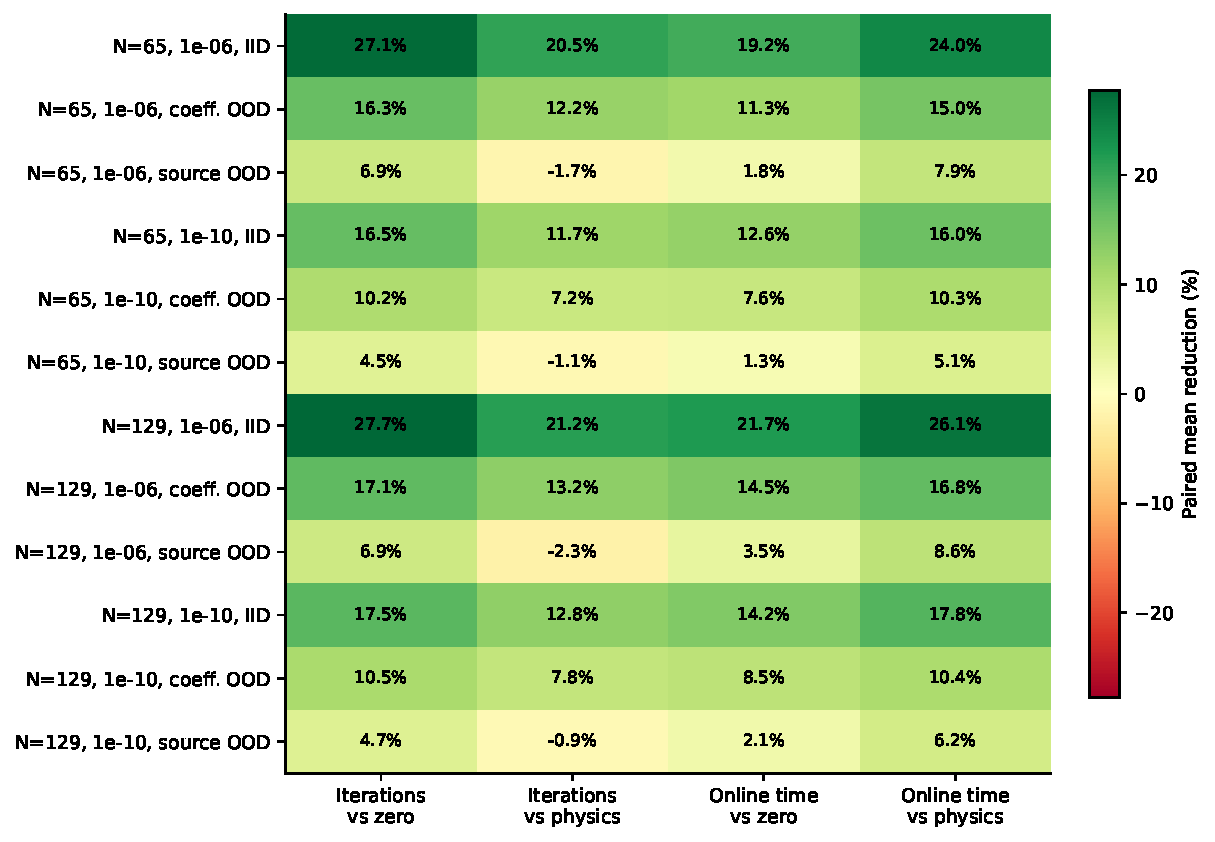
\includegraphics[width=.95\linewidth]{figures/matrix.pdf}
\caption{All S2 cells. Columns distinguish paired iteration and online-time reductions against zero and physics Laplacian starts. Negative values are retained.}\label{fig:matrix}
\end{figure}
\begin{figure}[ht]
\centering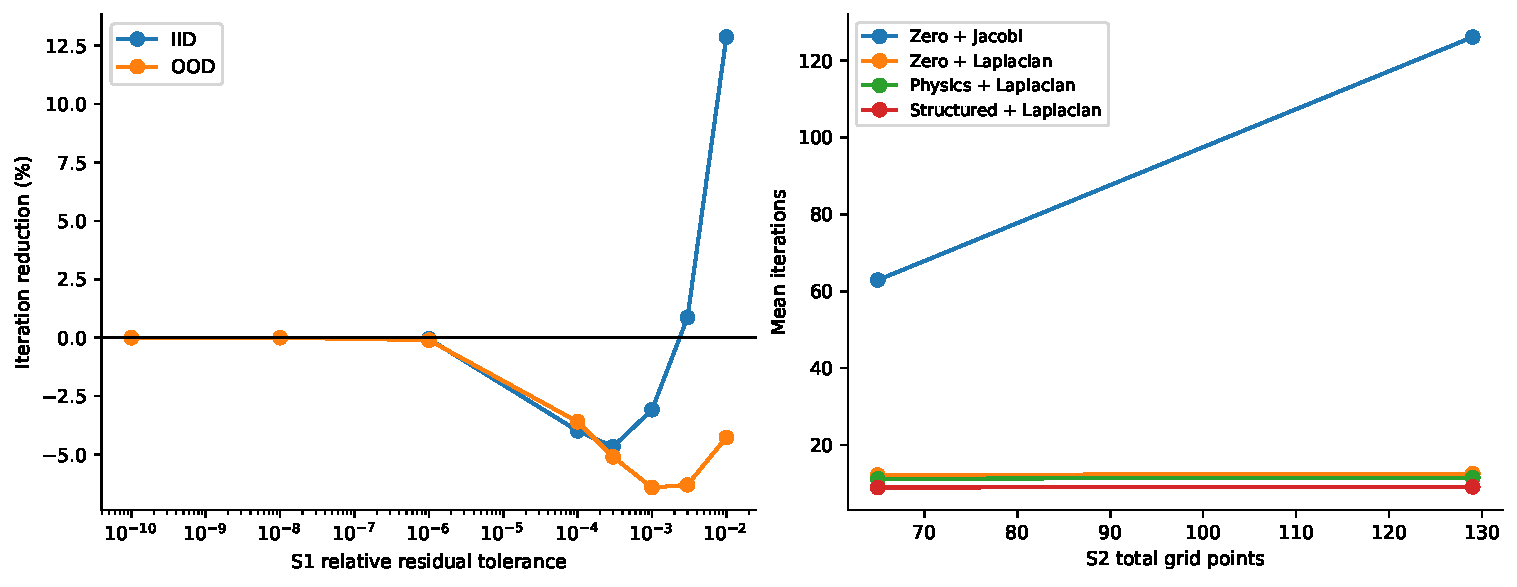
\includegraphics[width=\linewidth]{figures/tolerance_scaling.pdf}
\caption{Left: the development-only S1 tolerance diagnostic. Right: IID S2 iteration scaling at $10^{-6}$ with separately fitted models per grid. The two panels concern different, explicitly versioned studies.}\label{fig:sensitivity}
\end{figure}

\subsection{Resources and evidence verification}
The S2 producer records 175.59 CPU seconds, 175.75 wall seconds, and peak RSS 191.23 MiB before the subsequent verifier. These producer measurements exclude packaging, remote scheduling and later artifact replay. The runtime is Python 3.13.15 and NumPy 2.1.3 on Kaggle CPU with one BLAS/OpenMP thread. Offline fit and training-data generation measurements are retained per block, grid and model in \texttt{offline\_costs.json}; they are not hidden inside an assumed amortization.
